% This is samplepaper.tex, a sample chapter demonstrating the
% LLNCS macro package for Springer Computer Science proceedings;
% Version 2.20 of 2017/10/04
%
\documentclass[runningheads]{llncs}
%
\usepackage{graphicx}
\usepackage{tikz}
\usepackage{rotating}
\usepackage[pdftex,
            pdfauthor={Giuliano Belinassi, Richard Biener, Jan Hubicka and Alfredo Goldman},
            pdftitle={Compiling Files in Parallel: A Study with GCC},
            pdfsubject={Compiling in Parallel},
            pdfkeywords={Compilers, Parallel Compilation, Link Time Optimization, LTO},
            pdfproducer={LaTeX},
            pdfcreator={pdfTeX 3.14159265-2.6-1.40.21 (TeX Live 2020/Debian)}]{hyperref}

\usetikzlibrary{decorations.pathreplacing,shapes,arrows,positioning}
% Used for displaying a sample figure. If possible, figure files should
% be included in EPS format.
%
% If you use the hyperref package, please uncomment the following line
% to display URLs in blue roman font according to Springer's eBook style:
\renewcommand\UrlFont{\color{blue}\rmfamily}



\begin{document}
\bibliographystyle{plainurl}

%
\title{Compiling Files in Parallel: A Study with GCC\thanks{Supported by CAPES and Google Summer of Code.}}
%
%\titlerunning{Abbreviated paper title}
% If the paper title is too long for the running head, you can set
% an abbreviated paper title here
%
\author{Giuliano Belinassi\inst{1} \and Richard Biener\inst{2} \and Jan Hubi\v cka \inst{3} \and Alfredo Goldman\inst{1}}
%
\authorrunning{G. Belinassi et al.}
% First names are abbreviated in the running head.
% If there are more than two authors, 'et al.' is used.
%
\institute{Institute of Mathematics and Statistics, Rua do Matão 1010, São Paulo SP, BRA\\
\url{https://www.ime.usp.br} \and
SUSE Labs, Nürnberg 90409, GER\\
\url{https://www.suse.com/} \and
Charles University, Malostransk én ám. 25. 11800 Praha, CZE\\
\url{http://kam.mff.cuni.cz/}}

%
\maketitle              % typeset the header of the contribution
%
\begin{abstract}

Processors are becoming increasingly parallel, but compiling software has so
far been a task parallelizable only by the number of files in it. To improve
compilation parallelism granularity, we propose a method feasible to implement
in commercial compilers for single file parallel compilation, with simple
modifications in the Link Time Optimization (LTO) engine; which we show by
implementing it in GCC. This method resulted in a 35\% speedup when
self-compiling GCC when compared to \texttt{make -j} only parallelism, and
up to $3.5\times$ speedup when compiling individual files. 
We also explain why the adoption of our proposed method is still compatible
with the Reproducible Builds project.

\keywords{Compilers \and Parallel Compilation \and Link Time Optimization \and LTO.}
\end{abstract}
%
%
%
\section{Introduction}

The recent advances in both technological and computational fields induced an
increasingly faster expansion of software ecosystems. Developers create new
programs to supply the needs of the most diverse domains, either through web
systems coded in script languages; or by components to an operating system
destined to control some hardware resources. Regardless of the reason behind
the development of them, it is true that their code will be, at some
point, transformed into machine language by a compiler or assembler, even if an
interpreter executes it.

Compilers are enormous programs, largely adopted by industry and academia, where
a great effort has been employed to produce efficient code --
but without any sacrifice in correctness --. There are huge projects destined
to develop and improve them, such as the GNU Compiler Collections
(GCC)\footnote{https://gcc.gnu.org/} and LLVM\footnote{https://llvm.org/}, capable
of translating several languages such as C, C++, and Fortran, to machine language.

GCC was started by Richard Stallman, with the first public release in March of
1987, supporting the C language and targeting several architectures
\cite{gcc-first-ver}. Today, GCC is a multinational collaboration
project, with hundreds of thousands of lines of code, and perhaps the most used C/C++
compiler in the Linux ecosystem.

GCC was initially designed to compile programs one file at a time, meaning
that it could not allow global cross-file optimizations because the compiler
never had the opportunity to analyze the program as a whole. This scenario
changed when Link Time Optimization (LTO) was proposed \cite{gcc-lto,whoprgoogle} and
implemented \cite{glek2010optimizing}. GCC supports LTO by using
\texttt{-flto}. Part of the LTO engine has already been parallelized, which
inspired this work.

The main contribution of this work is to answer the question about how can we modify an
industrial scale compiler to compile single files in parallel. We address
that by reusing the already-existing LTO engine in it (in this
case, GCC) for partitioning the single file Translation Unit (TU) after the
Interprocedural Analysis (IPA) has been decided, and we proceed compiling
each partition individually, in parallel. IPA includes only interprocedural
optimizations, which requires interactions among distinct functions to optimize
(\emph{e.g.} inliner). There is already a way to instruct
the LTO engine to partition a single file TU by using
\texttt{-flto -flinker-output=nolto-rel}, but with phony object creation
overhead and no guarantee of correct name clash resolution, as discussed
in Section \ref{sec:name_clash_resolution}.

We present the previous efforts in compiling a single file in
parallel, as well as an introduction to LTO in Section \ref{sec:related}.
Then, we detail our work in single file compilation in
Section \ref{sec:work}, while exposing some internal mechanisms
of GCC. We then show how we ensured that our modifications are correct
in Section \ref{sec:methods}. Finally, we present our results in
Section \ref{sec:results} and discuss how to improve from this paper
in Section \ref{sec:future_works}.

\section{Related Works} \label{sec:related}

Parallel Compilation includes parsing (parallel or not), how to perform
analysis, optimization, and code translation in parallel.  Parsing can be
described as building a machine to decide if an input string is a member of a
certain language or not, creating the Abstract Syntax Tree in the process by
logging the used derivation rules.

Parallel Parsing dates back to 1970. Lincoln \cite{Lincoln:1970:PPT:987475.987478}
explored how to use the vectorial registers in the (so far)
STAR-100 supercomputer for lexical analysis. Fischer
\cite{fischer1975parsing} gives a detailed theoretical study, proving
several concurrent parsing techniques for the LR($k$) family.
The parser proceeds by breaking the input into several arbitrary parts, and running a
serial parser on each of them. Then the algorithm tries to
recover the stack of each noninitial parser by constructing a set of
possible states, for which there are 5 possible cases. However, in case
of an error, the parser result should be discarded, and therefore a lot
of work will be done in vain when comparing with the sequential version.

Fowler and Joshua \cite{fowler2009parallel} described how to parallelize Earley
and Packrat methods. For the former, the authors partition the Earley sets into
sub-blocks and run each block in parallel. For solving the dependency across
the blocks, the authors propose a way to speculate additional items into the
parser, which is not produced by the serial algorithm. For Packrat, the authors
propose a message passing mechanism.  The input is divided into parts, and each
part is assigned to a worker thread. Each thread speculates until the
thread on its left has finished parsing, and send the synthesized starting
symbol to the thread on its right. The authors managed a speedup of $5.5\times$
in Earley, and $2.5\times$ in Packrat.

Still on Packrat methods, Dubroy and Warth \cite{dubroy2017incremental} show
how to implement an incremental Pacrkat to avoids reparsing the entire input
on modifications. The authors achieve this by recording all its
intermediate results in a parsing table and modify the parsing program to reload
this table when invoked. The authors showed that their method does not require
any modification to the original grammar, and their method requires only
up to $11.7\%$ of extra memory when compared to the original parser. Authors
claim a reduction from $23.7ms$ to $6.2ms$ on reparsing a 279Kb input string.

Barenghi \textit{et al.} \cite{Barenghi:2015:PPM:2839536.2840146} explore
some properties of Operator Precedence Grammars to construct a Yacc-like
parser constructor named PAPAGENO, which generates parallel parsers. The
authors described precedence grammars for Lua and JSON, which they used in
their tests to get a speedup of up to $5.5\times$ when compared to a parser
generated by GNU Bison.

As for parallel compilation \textit{de facto}, works dates back from 1988.
Vandevoorde \cite{vandevoorde1988parallel} worked on a C compiler, and Wortman
and Junkin \cite{wortman1992} worked on a Modula-2+ compiler.  The former
assumes that every function declaration is in the file headers, and implements
per-function and per-statement parallel compilation. The latter implements only
per-function parallelism.  Speedups ranged from $1.5\times$ to $6\times$ on a
multicore MicroVAX II machine. None of these papers discuss optimization, and
they concentrate on (today's perspective) non-optimizer compilers, which are not
the case of GCC.

Lattner \emph{et al.} proposed MLIR, an Intermediate Representation (IR) which
aims to unify several Machine Learning frameworks and compilers IR \cite{mlir}.
Its design also includes support to multithreaded compilation by supporting
concurrent transversal and modification of the IR.

There has been an attempt of parallelizing GCC by threading the GIMPLE
intraprocedural pass manager \cite{bernardino2020improving}, which only
requires information contained inside the function's body (\textit{e.g.}
vectorization). The authors managed a speedup of up to $3.35\times$ to this
compilation stage, and up to $1.88\times$ in total compilation of a file when
extending this technique to the RTL passes.

\subsection{Link Time Optimization (LTO)} \label{lto_section}

Compilation usually uses the following scheme: a compiler consumes a source file,
generating an assembly file as output. This file is then assembled into an object file
and later linked with the remaining objects file to compose an executable or a library.
Fig. \ref{fig:gnu_toolchain} illustrates this process for a single file. In this paper,
we call this method the \emph{classical compilation} scheme.

\begin{figure}
\tikzstyle{block} = [rectangle, draw, fill=white,
    text width=6em, text centered, rounded corners, node distance=4.7cm, auto, minimum height=3em]
\tikzstyle{line} = [draw, -latex]
\tikzstyle{cloud} = [draw, ellipse,fill=white, node distance=2cm,
    minimum height=2em]
\makebox[\textwidth][c]{
\scalebox{0.8}{
\begin{tikzpicture}[node distance = 3cm, auto]
    % Place nodes
    \node [block]                      (cc1) {Compiler \\ (cc1)};
    \node [block, right of = cc1]      (as) {Assembler\\(as)};
    \node [block, right of = as]       (ld) {Linker};
    \coordinate [left of=cc1]          (fonte);
    \coordinate [right of=ld]    (bin);

    % Draw edges
    \draw[->]    (cc1.east)    -- (as.west)       node[midway, above] {Assembler File};
    \draw[->]    (cc1.east)    -- (as.west)       node[midway, below] {(.s)};
    \draw[->]    (as.east)     -- (ld.west)       node[midway, above] {Object File};
    \draw[->]    (as.east)     -- (ld.west)       node[midway, below] {(.o)};
    \draw[->]    (fonte.west)  -- (cc1.west)      node[pos=0, above] {Source File};
    \draw[->]    (fonte.west)  -- (cc1.west)      node[pos=0, below] {(.c)};
    \draw[->]    (ld.east)     -- (bin.west)      node[pos=1, above] {Executable};
\end{tikzpicture}
}
}%
\caption{GCC Compiling a .c file in \emph{classical compilation} mode}
\label{fig:gnu_toolchain}
\end{figure}

The issue around this scheme is that it can only optimize with
the information found in its TU because it can not see the body
content of other files' functions. A TU is the
entire content of a source file (a .c file in C) plus all its headers.

As an answer to this, LTO allows cross-module optimizations by
postponing optimizations and final translation to a linker wrapper. There, the entire
program can be loaded by the compiler (but more often, just some sort of summary)
as a single, big TU, and optimizations can be decided globally,
as now it has access to the internals of other modules. LTO is divided into
three steps \cite{whoprgoogle,glek2010optimizing}:
\begin{itemize}
\item LGEN (\textit{Local Generation}): each module is translated to an IR and
written to disk in phony object files. These objects are \emph{phony} because
they do not contain assembly code. This step runs serially on the input file
(\textit{i.e.} in parallel to the files in the project).

\item WPA (\textit{Whole Program Analysis}): load all translated modules,
merges all TUs into one, and analyzes the program globally. After that, it
generates an \emph{optimization summary} for the program and partitioned this
global TU for the next stage. This analysis runs sequentially to the entire
project.

\item LTRANS (\textit{Local Transformations}): apply the transformations generated by
WPA to each partition, which will generate its own object file. This stage runs in
parallel.
\end{itemize}

This process is sketched in Fig. \ref{fig:whopr_build}, where the linker
wrapper is represented by \textit{collect2}, which firstly launch \textit{lto1}
in WPA mode, and the second time it finally launches \textit{ld}. This process
can be seen by launching gcc with \texttt{-flto -v}.

\begin{figure}
\tikzstyle{block} = [rectangle, draw, fill=white,
    text width=6em, text centered, rounded corners, node distance=1cm and 0.5cm, minimum height=2em]
\tikzstyle{line} = [draw, -latex]
\makebox[\textwidth][c]{

\scalebox{0.8}{
\begin{tikzpicture}[node distance = 3cm, auto]
    % Place nodes
    \node [block]              (fonte1) {source1.c};
    \node [block, right= of fonte1]        (fonte2) {source2.cpp};
    \node [block, right= of fonte2]        (fonte3) {source3.f90};
    \node [block, above= of fonte2]         (make)   {Makefile};

    \node [block, below= of fonte1]        (gcc)      {gcc};
    \node [block, below= of fonte2]        (g++)      {g++};
    \node [block, below= of fonte3]        (gfortran) {gfortran};

    \node [block, below= of gcc]           (objeto1) {obj1.o};
    \node [block, below= of g++]           (objeto2) {obj2.o};
    \node [block, below= of gfortran]      (objeto3) {obj3.o};

    \node [block, below= of objeto2]       (gcc_lto) {collect2 (lto1)};

    \node [block, right= of fonte3]            (gcc_ltrans1) {gcc\_ltrans};
    \node [block, right= of gcc_ltrans1]   (gcc_ltrans2) {gcc\_ltrans};
    \node [block, right= of gcc_ltrans2]   (gcc_ltrans3) {gcc\_ltrans};

    \node [block, above= of gcc_ltrans2]       (gcc_wpa) {gcc\_wpa};
    \coordinate[below= of gcc_wpa]            (c2);


    \node [block, below= of gcc_ltrans1]   (obj1) {obj1.o};
    \node [block, below= of gcc_ltrans2]   (obj2) {obj2.o};
    \node [block, below= of gcc_ltrans3]   (obj3) {obj3.o};

    \node [block, below=of obj2]   (ld) {collect2 (LD)};

	\node [block, below=of ld]   (bin) {Binary};

    % Draw edges
    \draw[->]    ([xshift=-0.7em] make.south)   -- (fonte1.north);
    \draw[->]    (make.south)   -- (fonte2.north);
    \draw[->]    ([xshift=+0.7em] make.south)   -- (fonte3.north);

    \draw[->]    (fonte1.south)   -- (gcc.north);
    \draw[->]    (fonte2.south)   -- (g++.north);
    \draw[->]    (fonte3.south)   -- (gfortran.north);

    \draw[->]    (gcc.south)   -- (objeto1.north);
    \draw[->]    (g++.south)   -- (objeto2.north);
    \draw[->]    (gfortran.south)   -- (objeto3.north);

    \draw[->]    (objeto1.south)   -- ([xshift=-0.7em]gcc_lto.north);
    \draw[->]    (objeto2.south)   -- (gcc_lto.north);
    \draw[->]    (objeto3.south)   -- ([xshift=+0.7em]gcc_lto.north);

    %\draw[->]    (gcc_lto.south)   -- (gcc_wpa.north);
 	\draw[->]  (gcc_lto.east) .. controls +(6.5,0) and +(-6.5,0).. (gcc_wpa.west);

    \draw[->]    (gcc_wpa.south)   -- (gcc_ltrans1.north);
    \draw[->]    (gcc_wpa.south)   -- (gcc_ltrans2.north);
    \draw[->]    (gcc_wpa.south)   -- (gcc_ltrans3.north);

    \draw[->]    (gcc_ltrans1.south)   -- (obj1.north);
    \draw[->]    (gcc_ltrans2.south)   -- (obj2.north);
    \draw[->]    (gcc_ltrans3.south)   -- (obj3.north);

    \draw[->]    (obj1.south)   -- ([xshift=-0.7em]ld.north);
    \draw[->]    (obj2.south)   -- (ld.north);
    \draw[->]    (obj3.south)   -- ([xshift=+0.7em]ld.north);

	\draw[->]    (ld.south)   -- (bin.north);
	
	%draw brackets
\draw [decorate,decoration={brace,amplitude=10pt},xshift=-0.5cm,yshift=0pt]
([xshift=-1.3cm]objeto1.south) -- ([xshift=-1.3cm]fonte1.north) node [black,midway,xshift=-0.3cm]
{\footnotesize \begin{turn}{90}LGEN\end{turn}};

\draw [decorate,decoration={brace,amplitude=10pt},xshift=-0.5cm,yshift=0pt]
([xshift=1.3cm]gcc_ltrans3.north) -- ([xshift=1.3cm]obj3.south) node [black,midway,xshift=0.3cm]
{\footnotesize \begin{turn}{-90}LTRANS\end{turn}};


\draw [decorate,decoration={brace,amplitude=10pt},xshift=-0.5cm,yshift=0pt]
([xshift=1.3cm]gcc_wpa.north) -- ([xshift=1.3cm]gcc_wpa.south) node [black,midway,xshift=0.3cm]
{\footnotesize \begin{turn}{-90}WPA\end{turn}};


\end{tikzpicture}
}
}%
\caption{Compilation of a program using LTO scheme}
\label{fig:whopr_build}
\end{figure}

There are also papers using a profile-based approach rather than a whole-program
analysis for cross-module optimizations.  Xinliang \textit{et al.}
\cite{lipo} proposed LIPO, which embeds IPA in the generated
binary with minimal overhead, and loads information about functions in other
modules based on the profiling report. LIPO also removes the requirement of
phony object dumps and link time wrappers when compared to LTO. Results showed
a speedup of up to $10\times$ in compilation time when compared to Feedback
Driven Optimization (FDO) alone.

Following that, Johnson \textit{et al.} proposes ThinLTO \cite{thinlto}. It
differs from LTO by generating the function summaries on the LGEN stage for
improved parallelism, while avoiding the large memory footprint requirement on the
original LTO. ThinLTO also supports incremental builds by hashing the compiled
function to avoid recompilation of unmodified functions, while LTO requires
recompilation of the entire partition. Most GCC's IPA
optimizations only use summaries to avoid this memory footprint issue.


\section{Our Proposal} \label{sec:work}

As presented in Section \ref{lto_section}, LTO was created to allow
cross-module optimizations in programs, and has a serial part (WPA), imposing a
bottleneck on manycore machines. On the other hand, \emph{classical compilation}
scheme can not partition its TU for parallel
compilation, which can also be a bottleneck for the compilation if it is too large.
The latter issue, however, can be solved by transplanting the LTO partitioner
to the \emph{classical compilation} scheme and making it work \textit{without}
having the context of the \textit{entire} program. We claim that it is possible,
and show that by implementing it in GCC.

Our approach differs from LTO mainly in how we handle the IPA.
LTO handles these optimizations with the context of the whole program, while
our approach will only have the context of the original TU.
This allows optimizations as good as they are in the \emph{classical
compilation} scheme while benefiting from the extra parallelism opportunity
available in the LTO's LTRANS stage.

In this section, we will first discuss the internals of some parts of GCC,
which we had to modify for our implementation to work. In Subsection
\ref{sec:gcc_driver}, we present an important piece of the compiler from the
User Experience perspective: the \texttt{gcc} \textit{driver}. Then, in
Subsection \ref{sec:lto_partitioner} we present a short algorithm for making
the LTO partitioner work for our proposal. In Subsection
\ref{sec:partition_mask} we present a necessary change we had to do in our work
about how partitions are applied in GCC. In
Subsection \ref{sec:name_clash_resolution}, we explain how we solved the issue
of private symbols with the same name being promoted to global.
Then in Subsection \ref{sec:integration_jobserver}, we present an optional part
of our work about communicating with the GNU Make Jobserver to keep track of
used processors. And finally, we discuss why our proposal is still compatible
with the Reproducible Builds project in Subsection \ref{sec:repro_builds}.

\subsection{The \texttt{gcc} Driver}\label{sec:gcc_driver}

A large program can be written in several languages, with each of them having
its own compiler. From a compiler theory perspective, a compiler
translates a program from a language $A$ to another language $B$
\cite{dragonbook}. In GCC, it translates several languages to assembly
of some architecture (\textit{e.g.} x86). This means that
encapsulating code in object files, or linking these files in an executable, are
not tasks of the compiler. However, the user can launch \texttt{gcc -o binary
file.c} and get a working binary. That is because the binary \texttt{gcc} is
a \textit{driver}, and it will launch the
necessary programs for the user. In fact, this line launches three programs,
as illustrated in Fig. \ref{fig:gnu_toolchain}.

Therefore, if we want our changes do not break the building scripts
(\textit{e.g.}, Makefile) used by most projects -- which is mostly launching
\texttt{gcc file.c -c} which creates an object file \texttt{file.o} -- we must
ensure that we create a single object file for each file, not multiple, as does
the LTO partitioner. Fortunately, we can rely on GNU \textit{ld} partial linking
for merging objects file into one. Therefore, the solution to this problem is:
\begin{enumerate}
	\item Patch the LTO \textit{partitioner} to communicate the location of
	each created assembly file (.s) to the \textit{driver}. This can be
	done by passing a hidden flag \texttt{-fadditional-asm=<file>}
	by the driver to the partitioner, which the last will write to. This file can also
	be replaced with a Named Pipe for better performance if needed.

	Then, the partitioner checks if this flag has been passed to the compiler.
	If yes, then a \textit{compatible version} of the driver is installed. If
	the partitioner decides to partition the TU, it should \textit{retarget}
	the destination assembly file and write the retargeted name to the
	communication file.

	\item Patch the driver to pass this hidden flag to the
	\textit{partitioner}, and also to check if this file exists. If not, this means
	that either the compiler is incompatible or it has chosen not to partition
	the TU. In the first case, the driver should call the assembler to every
	assembly file generated, and call the linker to generate the expected
	final object file. In the second case, simply fallback to the previous
	compilation logic.
\end{enumerate}

Fig. \ref{fig:gnu_toolchain_patched} illustrates the code flow after these
changes.  The execution starts in the highlighted node \textit{gcc}, which
calls the compiler (cc1) with the necessary flags to establish a communication
channel among the parts. The compiler then will partition the TU and forks
itself into several child processes, one for each partition.

Once multiple processes are created, the compiler will communicate its output
.s file, and the driver then will launch the assembler (\textit{as}) to
generate several object files, and then launch the linker (\textit{ld}) to
merge them all into a single object file.

%After these changes, a good way to check if the changes are working is to
%bootstrap the compiler with a single partition, but writing the output
%path into the created communication channel. Bootstrapping can be a resource
%intensive task; therefore this is an excellent opportunity to write automated
%tests covering every case necessary for the bootstrap. This may also expose
%some extreme cases, for instance, the C compiler being called to process macros
%in files of distinct languages.

\begin{figure}
\tikzstyle{block} = [rectangle, draw, fill=white,
    text width=6em, text centered, rounded corners, minimum height=2em]
\tikzstyle{line} = [draw, -latex]

\makebox[\textwidth][c]{
\scalebox{0.8}{
\begin{tikzpicture}[node distance = 2.4cm, auto]
    % Place nodes
    \node [block]                      (cc1_1) {cc1};
    \coordinate [right= of cc1]          (c);
    \node [block, right= of c,fill={rgb:black,1;white,2}]        (driver1) {gcc};
    \node [block, above= of c]                      (cc1_2) {cc1};
    \node [block, below= of c]                      (cc1_3) {cc1};
    \coordinate [above= of driver1]          (c2);
    \coordinate [below= of driver1]          (c3);
    \node [block, right= of c2]      (as2) {as};
    \node [block, right= of c3]      (as3) {as};
    \node [block, right= of driver1]       (ld) {ld};
    \coordinate [left= of cc1]          (fonte);
    \coordinate [right= of ld]    (bin);

    % Draw edges
    \draw[->]    (driver1.west)    -- (cc1_1.east) node[midway, above] {\texttt{-fadditional-asm=<file>}};
    \draw[->]    ([xshift=+0.5cm]cc1_2.south) -- ([xshift=-0.5cm]driver1.north) node[midway, above, sloped] {Generates .s file};
    \draw[->]    ([xshift=+0.5cm]cc1_3.north) -- ([xshift=-0.5cm]driver1.south) node[midway, above, sloped] {Generates .s file};

    \draw[->]    (cc1_1.north)    -- ([xshift=-0.5cm]cc1_2.south) node[midway, above, sloped] {Forks};
    \draw[->]    (cc1_1.south)    -- ([xshift=-0.5cm]cc1_3.north) node[midway, above, sloped] {Forks};

    \draw[->]    ([xshift=+0.5cm]driver1.north)  -- (as2.south) node[midway, above, sloped] {Assemble received .s};
    \draw[->]    ([xshift=+0.5cm]driver1.south)  -- (as3.north) node[midway, above, sloped] {Assemble receibed .s};
    \draw[->]    (driver1.east)  -- (ld.west) node[midway, above, sloped] {Links};

%    \draw[->]    (cc1.east)    -- (as.west)       node[midway, above] {Assembler File};
%    \draw[->]    (cc1.east)    -- (as.west)       node[midway, above] {Assembler File};
%
%    \draw[->]    (cc1.east)    -- (as.west)       node[midway, below] {(.s)};
    \draw[->]    ([xshift=+0.5cm]as2.south)     -- (ld.north)       node[midway, above, sloped] {Object File};
    \draw[->]    ([xshift=+0.5cm]as3.north)     -- (ld.south)       node[midway, below, sloped] {Object File};
%    \draw[->]    (fonte.west)  -- (cc1.west)      node[pos=0, above] {Source File};
%    \draw[->]    (fonte.west)  -- (cc1.west)      node[pos=0, below] {(.c)};
    \draw[->]    (ld.east)     -- (bin.west)      node[pos=1, above] {\texttt{file.o}};
\end{tikzpicture}
}
}%
\caption{Interaction between the \textit{driver}, the \textit{compiler}, and other tools
after our changes}
\label{fig:gnu_toolchain_patched}
\end{figure}

\subsection{Adapting the LTO Partitioner}\label{sec:lto_partitioner}

In GCC, a TU is represented as a callgraph. Every function, global variable, or
clones (which may represent a function to be inlined) is represented as nodes
in a callgraph. If there is a function call from $f$ to $g$, or there is a
reference to a global variable $g$ in $f$, then there is an edge from $f$ to
$g$. This means that TU partitioning can be represented as a \emph{graph
partitioning} problem.

When LTO is enabled and GCC is in the WPA stage, the body of these nodes
is not present, just a \textit{summary} of them (\textit{e.g.} the size
in lines of code it had). This is done to save memory. However,
when LTO is disabled, the function body is present, resulting
in some assertion failures, which were fixed after some debugging.

Then comes the partitioner algorithm \textit{de facto}. In LTO, GCC tries to
create partitions of similar size, and always try to keep nodes together. The
heuristic used by the original partitioner runs in linear time, and because of
that its code is quite complex. This resulted in a difficult process of finding
and solving the issues causing a partitioning failure, and therefore, we
decided to design a new partitioning algorithm for this project.

This partitioning algorithm works as follows: for each node, we check if it
is a member of a COMDAT \cite{comdat} group, and
merged it into the same partition. We then propagate outside of this COMDAT group;
checking for every node that may trigger the COMDAT to be copied into other
partitions and group them into the same partition. In practice,
this means to include every node hit by a Depth-First
Search (DFS) from the group to a non-cloned node outside of the group.
Fig. \ref{fig:comdat_frontier} represents a sketch of this process.

\begin{figure}
\centering
	 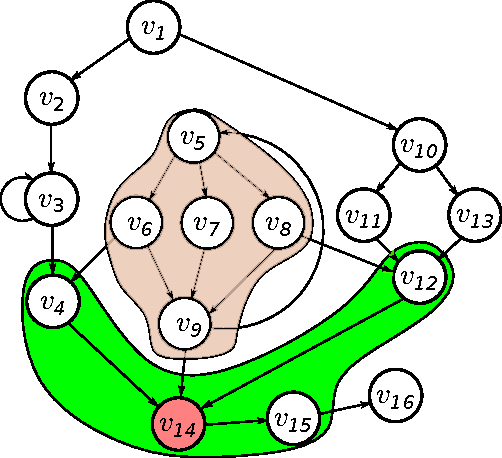
\includegraphics[scale=0.7]{figuras/comdat_frontier.pdf}
	  \caption{Example of callgraph, in beige being represented the COMDAT group,
	  in green the COMDAT frontier, and in red the cloned nodes.}
	  \label{fig:comdat_frontier}
\end{figure}

At first, we also did this process for private functions to avoid
promoting them to public, once external access would be necessary if they go
into distinct partitions. However, results showed that this has a strong
negative hit in any parallelism opportunity.

For grouping the nodes together,
we used a Union Find with Path Compression, which yields an attractive
computational complexity of $O(E + N \lg^*N)$ to our partitioner, where $N$ is the
number of nodes and $E$ is the number of edges in the callgraph \cite{feufiloff}.

Once the partitions are computed, we need to compute its \textit{boundary}.
If function $f$ calls $g$, but they were assigned into distinct partitions,
then we must include a version of $g$ in $f$'s partitions without its body,
then check if $g$ is a private function. If yes, then $g$ must be promoted
to a public function. There is also extra complexity if a version of $g$
is marked to be inlined in $f$, which means that its body has to be
streamed somehow. Fortunately, most of this logic is already present
in LTO and we could reuse them. However, some issues were found
when handling inline functions and global variables marked as part
of the boundary. First, some functions marked to be inlined into 
functions inside the partition were incorrectly marked to be removed.
Second, being variables marked as in the boundary (and therefore
not in the partition) not being correctly promoted to external. The reason
for these issues was hard to find the reason of, but easy to fix.

Furthermore, there were some issues concerning how GCC handles
partitions, which we discuss in the next subsection.

\subsection{Applying a Partition Mask}\label{sec:partition_mask}

Once partitions are computed, the only presented way to apply it
(\textit{i.e.}, remove every unnecessary node from the TU) was to reload the
compiler and let it load the phony object files. The issue is that these
objects are not available in our project because we are not running in LTO
mode. We developed another method for this.
We used the Unix \textit{fork} function to spawn a child process, and then
we implemented our own method to apply the partition without having to load
these phony object files. Fortunately, this consisted
of four cases:
\begin{itemize}
	\item \textit{Node is in partition}: nothing has to be done.
	\item \textit{Node is in boundary, but keep its body}: we mark that this function
	is available in other partitions, but we do not release its body or
	data structures.
	\item \textit{Node is in boundary}: we mark this mode as having its body removed,
	but we never actually remove it. This is because the node may share the
	body contents with another node in the partition. We then remove
	every edge from its functions to its callees, all references to variables,
	the content of the Dominator Tree, and also its Control-Flow Graph. This
	is now a function which this partition only know that it exists.
	\item \textit{Node not in boundary}: we remove the node and all its content.
\end{itemize}

After this, it retargets the output assembly file to another file private to
this partition and writes a pair (\textit{partition number, path to file}) into the
communication file, which the driver will read in the future. The partition
number is important to guarantee that the build is reproducible, as we will
discuss later.

It is also important that some early step in the compiler does not emit assembly
too early, such as the issue with the gimplifier in GCC, or else the output
file will be incomplete. We had to fix the gimplifier to avoid that.

Once the partition is applied to the child process, and the output file has
been communicated to the driver, it can continue with the compilation. It
should be running in parallel now by the number of partitions.

\subsection{Name Clash Resolution}\label{sec:name_clash_resolution}

In LTO, if there are two promoted symbols to global with the same (mangled) name, a
straightforward way to fix that is to increment a counter for each clashed
symbol. This is possible because LTO has the context of the entire program,
which we do not. Therefore, we need another way of fixing it.

Two naive approaches would be to select a random integer and append to the
function's name, or append the memory address of the function object to the
function's name.  Both of them breaks bootstrap \cite{bootstrap}, the first
because output functions will have distinct names on every new compilation. The
second because stage 1 compiles with \texttt{-O0} and stage 2 with
\texttt{-O2}, which changes the memory address of the functions between these stages.

Our solution is to use a crc32 hash of the original file and append it to the
function's name.  There is still a tiny probability of name clash with this
approach, however, we did not find any on our tests.

\subsection{Integration with GNU Make Jobserver}\label{sec:integration_jobserver}

GNU Make can launch jobs in parallel by using \texttt{make -j}.  To
avoid unnecessary partitioning and job creation when the CPU is at 100\% usage,
we have also implemented an integration mechanism with GNU Jobserver
\cite{posixjobserver}.  The implementation is simple: we query the server for
an extra token. If we receive the token, then it means that some processor is
available, and we can partition the TU and launch jobs inside the compiler.
Else, the processor workload is full, and it may be better to avoid
partitioning altogether.

However, for a program to be able to communicate with the jobserver, it should
be launched with a prepended \texttt{+} character (\textit{e.g.} $\texttt{+gcc
-c file.c}$), and therefore it is not so straightforward to use this mode on
existing projects.

\subsection{Relationship with Reproducible Builds}\label{sec:repro_builds}

One interesting point of Open Source is that it can be verified by everyone.
However, very often these projects are distributed in a binary form to the
users, removing from them the burden of this process. But nothing avoids that a
malicious developer modifies the codebase \textit{before} the distribution
(\textit{e.g.} inserting a backdoor), and claiming that he/her got a distinct
binary because his/her system is different from the user.

The Reproducible Builds project aims to solve that issue by providing a way to
reproduce the released binary from its source. Some software needs to
be patched to work with Reproducible Builds, for instance,
to not contain some kind of build timestamp, and so on. A build
is called \textit{reproducible} if given the same source code and build
instructions, anyone can recreate a bit-perfect version of the distributed
binary \cite{reproducible_builds}.

To keep compatibility with this project, we must ensure that our compiler
always outputs the same code with a given input. The input is not only
the source file itself but also the flags passed to it.

We claim that our modification still supports the Reproducible Builds because
of the following reasons:

\begin{itemize}
	\item No random information is necessary to solve name clashing.
	\item Given a number of jobs, our partitioner will always generate
	the same number of partitions for a certain program, always with the same content.
	\item Partial Linking is always done in the same order. To ensure that,
	we communicate to the driver a pair (\textit{partition number, path to file}),
	and we sort this list using the partition number as the key.
	\item No other race conditions are introduced, as we rely on the quality of
	the LTO implementation of the compiler.
\end{itemize}

However, there is one point of concern, which is the Jobserver Integration.  If
the processor is already in 100\% usage, we avoid partitioning at all and
proceed with sequential compilation. This certainly changes accordingly to the
processor usage of the machine during the build, therefore the build is not
guaranteed to be reproducible if this option is enabled. This is not an issue
if the number of jobs is determined beforehand.

\section{Methods}\label{sec:methods}

We ensure the correctness of our changes by (1) bootstrapping GCC; (2) ensure
that the GCC testsuite was passing; and (3) compiling random programs generated
with \textit{csmith} \cite{csmith} and ensure that the correct result was
found. These tests were done with 2, 4, 8 and 64 parallel jobs, with minimum
partitioning quota of $10^3$ and $10^5$ instructions.

For the time measurements, all points represent the average of collected
samples, with errorbar representing a $95\%$ confidence interval.
Our test files consisted of preprocessed source files from GCC, which compiles
without external includes. We collected $n = 15$ samples for every one of these
files. For the projects, we collected $n = 5$ samples because compilation is a
computer intensive task. We made sure that in every test, \texttt{-g0} was passed
for fairness, once there is a bug in our branch regarding debug symbols of
nodes in other partitions.

Tests were mainly executed in two computers, which are represented
in Table \ref{table:machines}. The graphic caption specifies where the test
was run.

The version of GCC used in the tests is available in the \texttt{autopar\_europar\_2021}
branch of \texttt{git://gcc.gnu.org/git/gcc.git}, with hash \texttt{e2da2f7205}.

%We ensure the correctness of our changes by:
%\begin{enumerate}
%	\item Bootstraping GCC with the number of parallel jobs as
%	2, 4, 8 and 64, with minimum partitioning quota of $10^3$ and $10^5$
%	instructions. We found issues with regard 
%
%	\item Run the GCC testsuite, which we noticed that all tests related to the debug
%	symbols were failing. However, if \texttt{-g0} is passed, no debug symbol is created,
%	and the bug related to this issue is never triggered. The reason behind this is
%	because our partition applier do not remove the symbols associated with removed
%	nodes, resulting in unknown symbol being dumped into assembler.
%
%	\item Generated random programs with \textit{csmith} \cite{yang2011finding}. This found more complicated
%	bugs (for instance, long strings being output before the assembler file retarget),
%	which we fixed.
%\end{enumerate}

\begin{table}[]
\centering
\begin{tabular}{c|c|c|c|c|}
\cline{2-5}
                                      & Number of Cores & Number of Threads & RAM                                                    & Storage Device \\ \hline
\multicolumn{1}{|c|}{Core-i7 8650U}   & 4               & 8                 & \begin{tabular}[c]{@{}c@{}}8Gb\end{tabular} & SSD       \\ \hline
\multicolumn{1}{|c|}{4x Opteron 6376} & 32              & 64                & \begin{tabular}[c]{@{}c@{}}252Gb\end{tabular}   & HDD       \\ \hline
\end{tabular}
\caption{Machine specification of tests}
\label{table:machines}
\end{table}

\vspace*{-1cm}

\section{Results}\label{sec:results}

We first highlight our best results in Table \ref{table:files}. On this table,
the autogenerated column means that this file is compiled to C++, and then compiled
into assembly by GCC. We managed speedups of up to a $2.4\times$ on Core-i7 when
compiling individual files with 8 threads, and up to $3.53\times$ on Opteron 6376 when
with 64 threads. Fig. \ref{fig:gcc_all_files} shows the results
of all files in GCC. Here we can see that for files with $\textit{Number of Instructions} >
1 \times 10^5$, we have mostly significant improvements.

We will now discuss how our proposed changes impact the overall compilation
time of some projects. For this, we run experiments compiling
the Linux Kernel 5.19.6, Git 2.30.0, the GCC version mentioned in
Section \ref{sec:methods} with and without bootstrap enabled, and JSON C++, with
commit hash \texttt{01f6b2e7418537}. We have only enabled jobserver integration
in GCC and Git, because it is necessary to modify an absolute large number
of Makefiles to do so (for instance, Linux has 2597 Makefiles).

In Fig. \ref{fig:gcc_projects} we show our results. We can observe a near
$35\%$ improvement when compiling GCC with bootstrap disabled, $25\%$ when
bootstrap is enabled, and $15\%$ improvement when compiling Git compared to
\texttt{make -j64} alone. Our jobserver implementation also squeezed a small
improvement in GCC compilation, but showed a massive slowdown in Git. This is
because Jobserver integration has interprocess communication cost
with Make, which is a problem if the size of the partitions is small.  These
tests were executed with 64 Makefile jobs and 8 threads inside the compiler.
Other than this, we seen no significant speedup or slowdown in these other
projects.

\begin{table}[]
\makebox[\textwidth][c]{
\begin{tabular}{l|c|c|c|c|c|c|c}
\cline{2-7}
                                       & \multicolumn{3}{c|}{Core-i7}     & \multicolumn{3}{c|}{Opteron 6376}                                                                & \multicolumn{1}{l}{}               \\ \hline
\multicolumn{1}{|l|}{File}             & Sequential & 8 Threads & Speedup & \multicolumn{1}{l|}{Sequential} & \multicolumn{1}{l|}{64 Threads} & \multicolumn{1}{l|}{Speedup} & \multicolumn{1}{c|}{Autogenerated} \\ \hline
\multicolumn{1}{|l|}{gimple-match.c}   & $76s$        & $31s$       & $2.4\times$     & $221s$                            & $66s$                             & $3.32\times$                         & \multicolumn{1}{c|}{yes}           \\ \hline
\multicolumn{1}{|l|}{insn-emit.c}      & $23s$        & $10s$       & $2.25\times$    & $97s$                             & $37s$                             & $3.53\times$                         & \multicolumn{1}{c|}{yes}           \\ \hline
\multicolumn{1}{|l|}{tree-vect-stmt.c} & $11s$        & $5s$        & $2.14\times$    & $32s$                             & $13s$                             & $2.46\times$                         & \multicolumn{1}{c|}{no}            \\ \hline
\end{tabular}
}
\caption{Speedup of highlighted files}
\label{table:files}
\end{table}

\begin{figure}
\centering
	 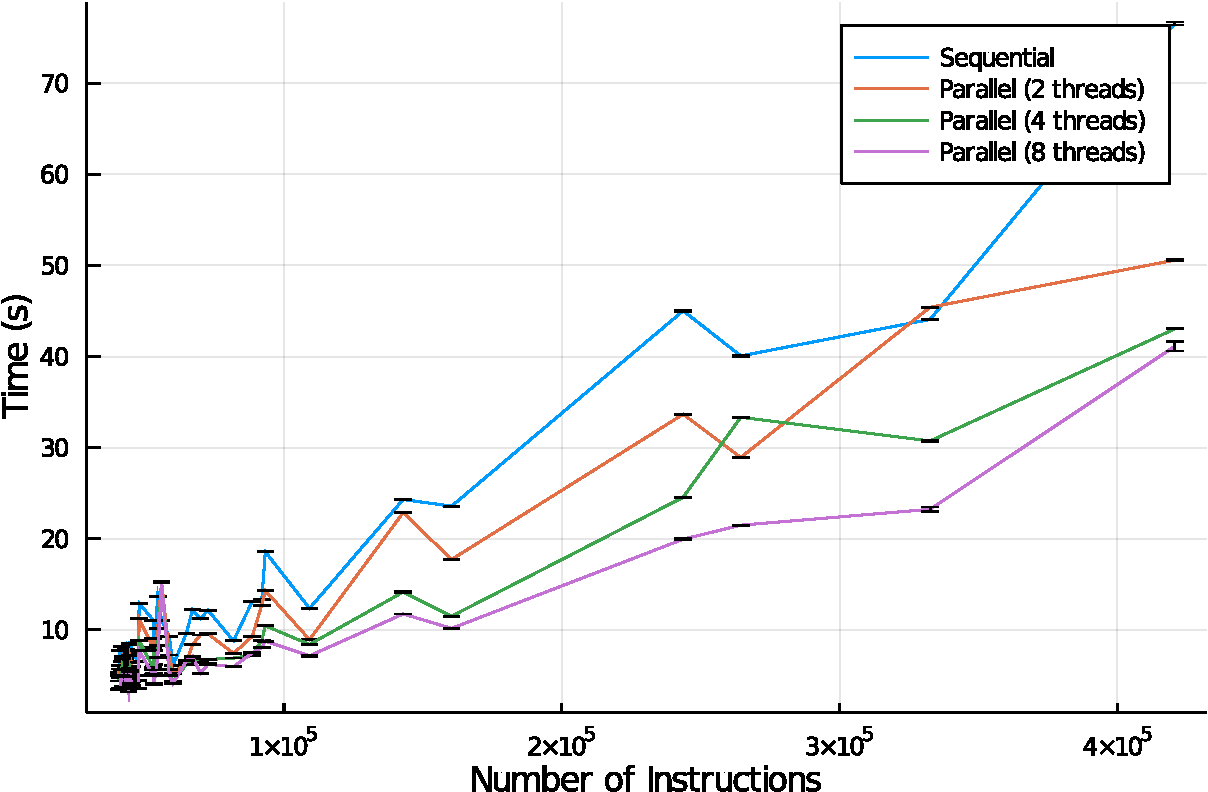
\includegraphics[scale=0.6]{figuras/times-insns-crop.pdf}
	  \caption{Compilation of each file with 1, 2, 4, and 8 threads on
	  Core-i7}
	  \label{fig:gcc_all_files}
\end{figure}

\begin{figure}
\centering
	 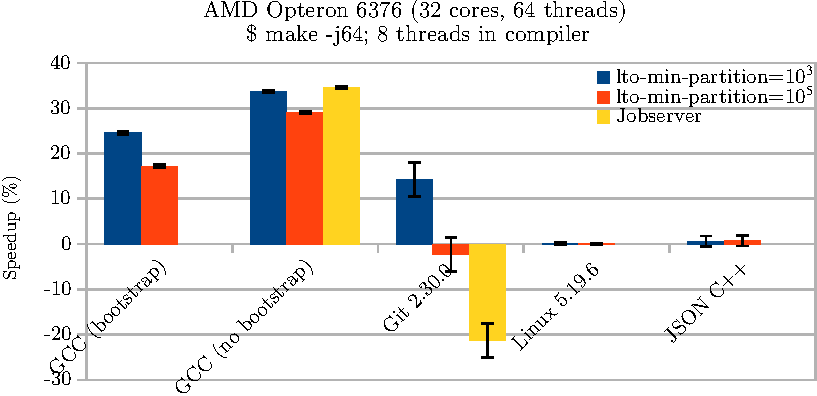
\includegraphics[scale=0.85]{figuras/experiment_projects_new-crop.pdf}
	  \caption{Compilation of some projects with 64 Makefile jobs and 8 threads in compiler in Opteron 6376}
	  \label{fig:gcc_projects}
\end{figure}

\section{Conclusions, Issues, and Future Works}\label{sec:future_works}

We have shown a tangible way of compiling files in parallel capable
of being implemented in industrial compilers, which resulted in
speedups when compiling single files in parallel, as well as some
speedup when compiling entire projects in manycore machines. However,
There are several points in which our work can be improved.

First is by fixing the bugs which is already known. There is (1) a bug related
to how our partitioner applier handle nodes created by the \textit{ipa-split}
pass, and therefore we have disabled it for now; and (2) our partitioner
applier do not remove debug symbols associated with removed nodes, resulting in
unknown symbols being dumped into the final assembly. These bugs certainly prevents the
current branch from being used in industrial environments (which is a good
reason why this was not merged in upstream yet), but they are fine as a proof
of concept to support our claims.

Second is by implementing a better partitioner to the project. One main issue
with our partitioner is that we kept its load balancing algorithm minimal to
ensure that it works. Using the LTO default partitioner as a base is a good start.

Third, by modifying the driver to also support external compiler through GCC
SPEC language. Our current implementation only checks if launching program
is a known compiler/assembler/linker, and will get confused in languages that
needs additional steps (such as CUDA).

Forth, try to develop a predictive model to decide if the input file is
a good candidate for parallel compilation. Fig. \ref{fig:gcc_all_files} shows
a clear linear correlation between the expected number of instructions and time
(and maybe it is the best parameter), but it may be possible to (statically)
collect more information about the file for a better decision.

And fifth, try to avoid partial linking and symbol promotion altogether
by concatenating the generated assembly files, instead of linking every
generated assembly file into temporary object files.

We also would like to draw attention to LTO's WPA step, which still runs
sequentially. Parallelizing this step, which includes all IPA passes would
improve parallel compilation of projects across the board in both LTO mode and
in our work. Profiling shows us that $11\%$ of the compilation time is spent in
this mode, while our project parallelized $75\%$ of the compiler.

%
% ---- Bibliography ----
%
% BibTeX users should specify bibliography style 'splncs04'.
% References will then be sorted and formatted in the correct style.
%
% \bibliographystyle{splncs04}
% \bibliography{mybibliography}
%
%\begin{thebibliography}{8}
%\bibitem{ref_article1}
%Author, F.: Article title. Journal \textbf{2}(5), 99--110 (2016)
%
%\bibitem{ref_lncs1}
%Author, F., Author, S.: Title of a proceedings paper. In: Editor,
%F., Editor, S. (eds.) CONFERENCE 2016, LNCS, vol. 9999, pp. 1--13.
%Springer, Heidelberg (2016). \doi{10.10007/1234567890}
%
%\bibitem{ref_book1}
%Author, F., Author, S., Author, T.: Book title. 2nd edn. Publisher,
%Location (1999)
%
%\bibitem{ref_proc1}
%Author, A.-B.: Contribution title. In: 9th International Proceedings
%on Proceedings, pp. 1--2. Publisher, Location (2010)
%
%\bibitem{ref_url1}
%LNCS Homepage, \url{http://www.springer.com/lncs}. Last accessed 4
%Oct 2017
%\end{thebibliography}

\bibliographystyle{splncs04}
\bibliography{bibliography}

\end{document}
